\documentclass[11pt,dvipdfmx,b5paper,oneside,report]{jsbook}

\usepackage{color}
\usepackage{here}
\usepackage{framed}
\usepackage{tcolorbox}
\usepackage{quotchap}
\usepackage{pdfpages}
\usepackage[hidelinks]{hyperref}
\usepackage{pxjahyper}
\usepackage{titlesec}
\usepackage{picture}
\usepackage{tikz}
\usepackage{graphicx}
\usepackage{geometry}

\tcbuselibrary{breakable}
\definecolor{shadecolor}{gray}{0.80}



% section
\titleformat{\section}[block]{}{}{0pt}
{
  \definecolor{teal}{gray}{0.30}
  \begin{picture}(0,0)
    \put(-10,-5){
      \begin{tikzpicture}
        \fill[teal] (0pt,0pt) rectangle (5pt,19pt);
      \end{tikzpicture}
    }
    \put(-10,-5){
      \color{teal}
      \line(1,0){\hsize}
    }
  \end{picture}
  \hspace{0pt}
  \sf \Large \thesection
  \hspace{0pt}
}

% 図表見出し
\renewcommand{\tablename}{\textcolor{gray}{▼} 表}
\renewcommand{\figurename}{\textcolor{gray}{▲} 図}

\begin{document}

\begin{titlepage}
  \newgeometry{left=0cm,right=0cm,top=0cm,bottom=0cm}
  \centering
  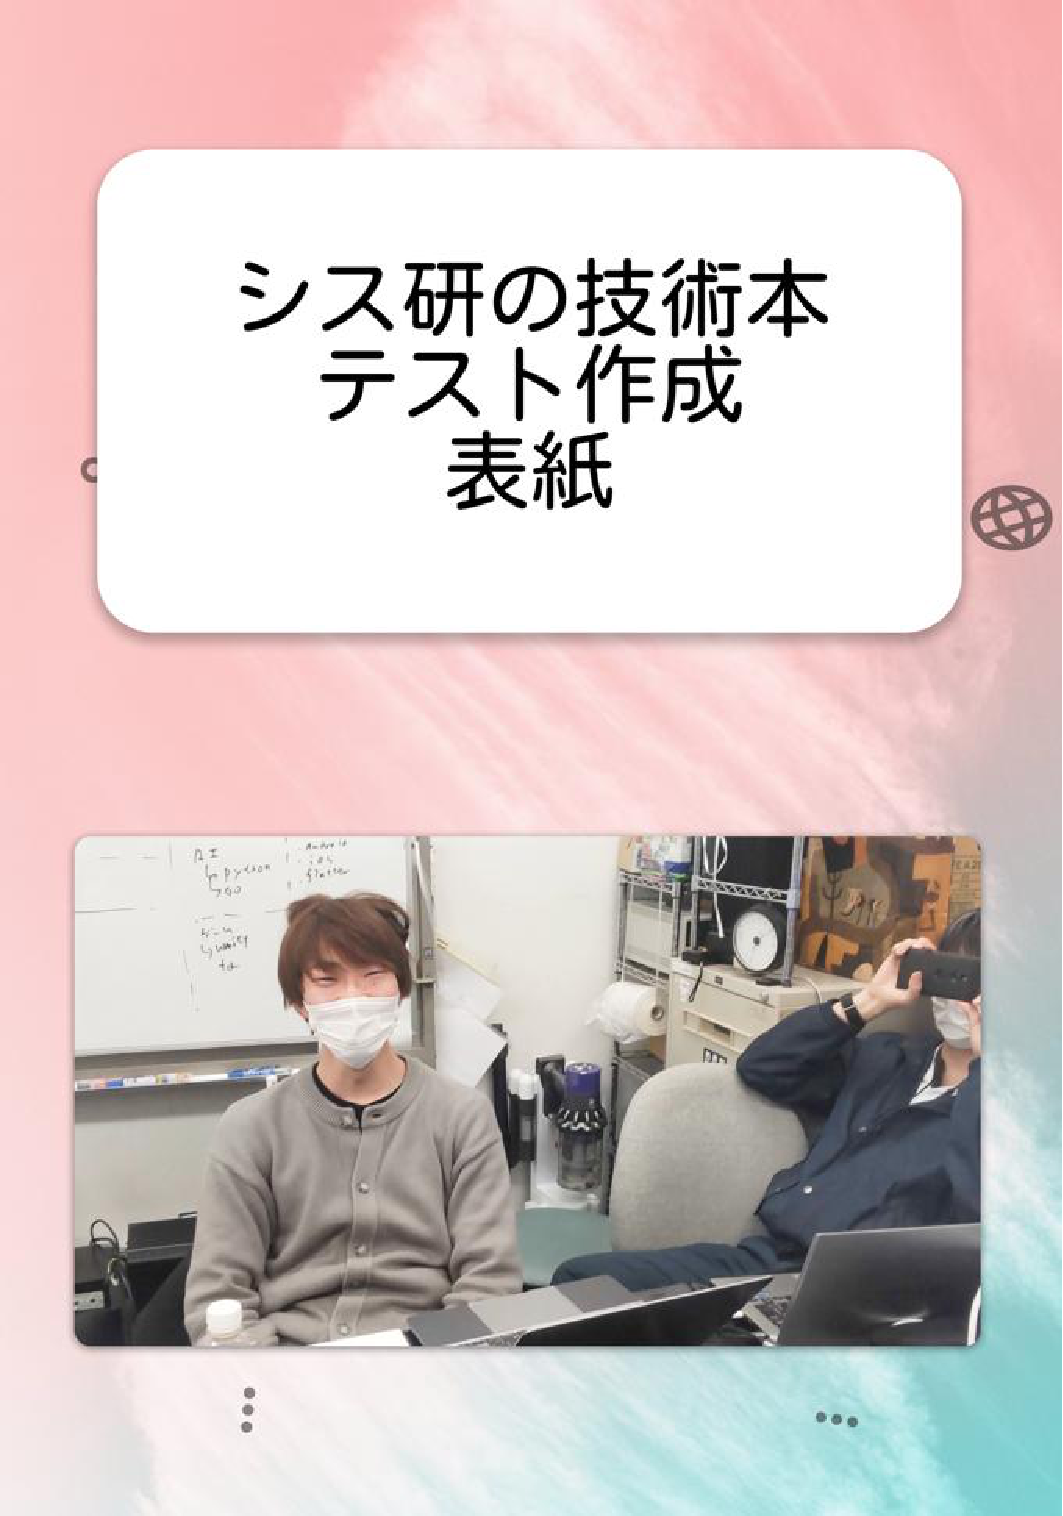
\includegraphics[width=\paperwidth,height=\paperheight]{image/titlepage.png}
  \restoregeometry % 元の余白に戻す
\end{titlepage}

%目次を自動的に作る。
\tableofcontents

\chapter{これはchapter}
\section{これはsection}
走れメロス
太宰治

メロスは激怒した。必ず、かの邪智暴虐じゃちぼうぎゃくの王を除かなければならぬと決意した。
メロスには政治がわからぬ。メロスは、村の牧人である。笛を吹き、羊と遊んで暮して来た。
けれども邪悪に対しては、人一倍に敏感であった。きょう未明メロスは村を出発し、野を越え山越え、十里はなれた此このシラクスの市にやって来た。
メロスには父も、母も無い。女房も無い。十六の、内気な妹と二人暮しだ。
この妹は、村の或る律気な一牧人を、近々、花婿はなむことして迎える事になっていた。
結婚式も間近かなのである。
メロスは、それゆえ、花嫁の衣裳やら祝宴の御馳走やらを買いに、はるばる市にやって来たのだ。
先ず、その品々を買い集め、それから都の大路をぶらぶら歩いた。メロスには竹馬の友があった。
セリヌンティウスである。今は此のシラクスの市で、石工をしている。その友を、これから訪ねてみるつもりなのだ。
久しく逢わなかったのだから、訪ねて行くのが楽しみである。歩いているうちにメロスは、まちの様子を怪しく思った。
ひっそりしている。
もう既に日も落ちて、まちの暗いのは当りまえだが、けれども、なんだか、夜のせいばかりでは無く、市全体が、やけに寂しい。のんきなメロスも、だんだん不安になって来た。
路で逢った若い衆をつかまえて、何かあったのか、二年まえに此の市に来たときは、夜でも皆が歌をうたって、まちは賑やかであった筈はずだが、と質問した。
若い衆は、首を振って答えなかった。しばらく歩いて老爺ろうやに逢い、こんどはもっと、語勢を強くして質問した。
老爺は答えなかった。メロスは両手で老爺のからだをゆすぶって質問を重ねた。
老爺は、あたりをはばかる低声で、わずか答えた。



\chapter{これはchapter}
\section{これはsection}
我輩は猫である\footnote{こんな感じで脚注を書く}。

どこで生れたかとんと見当がつかぬ。何でも薄暗いじめじめした所でニャーニャー泣いていた事だけは記憶している。吾輩はここで始めて人間というものを見た。しかもあとで聞くとそれは書生という人間中で一番獰悪な種族であったそうだ。この書生というのは時々我々を捕えて煮て食うという話である。

\begin{tcolorbox}[breakable]
\begin{verbatim}
1  /* ここにはソースコードを書く */
2  #include<stdio.h>
3
4  int main(void)
5  {
6    printf("Hello, World!\n");
7    return 0;
8  }
9  /* breakableを付けるとこんな感じで改行にも対応できる */
\end{verbatim}
\end{tcolorbox}

\begin{shaded}
\begin{verbatim}
## ここにはコマンドを書く
$ echo "Hello, World!"
\end{verbatim}
\end{shaded}

図表はキャプションを付けたときに、先頭に「▲」や「▼」を付けるようにした。

\begin{table}[H]
  \centering
  \caption{表のサンプル}
  \begin{tabular}{|c|l|l|l|} \hline
    日本 & hoge & fuga & piyo \\ \hline
    アメリカ & foo & bar & baz \\ \hline
  \end{tabular}
  \label{table-sample1}
\end{table}

\begin{figure}[H]
  \centering
  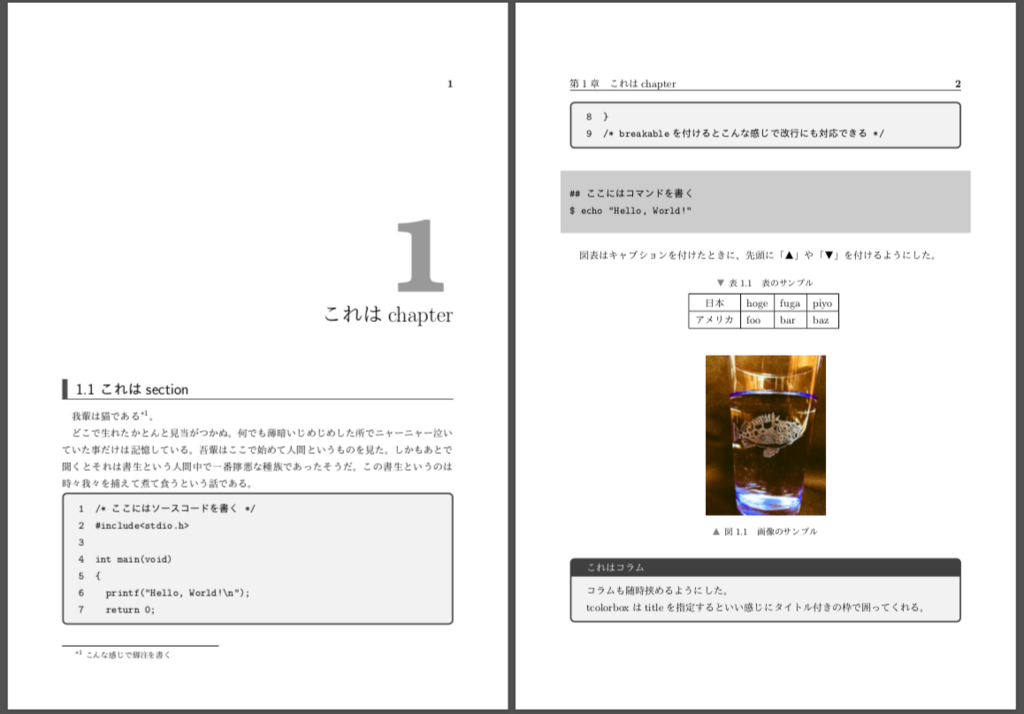
\includegraphics[width=4cm]{image/sample.png}
  \caption{画像のサンプル}
  \label{figure-sample1}
\end{figure}

\begin{tcolorbox}[title=これはコラム]
  コラムも随時挟めるようにした。

  tcolorboxはtitleを指定するといい感じにタイトル付きの枠で囲ってくれる。
\end{tcolorbox}


\end{document}